\chapter{Topology}

\section{Mapping}
So far we have seen how to construct sets, compare sets, and find `relations' between the elements of set. A natural extension are functional maps that take entire (sub)sets to different (sub)sets. A mapping, in this sense, is an abstract function which operates on sets by taking its individual elements to another set. This way, functional maps allow us to talk about comparisons of sets, relate sets, and to \textit{transform} one set to the other.

\begin{definition}
We define a \textbf{mapping} from a set $A$ to a set $B$ by any relation that takes the elements of $A$ to result in an element of $B$. It is denoted as $f:A\rightarrow B$ and for some $a\in A,a \mapsto f(a)$.
Suppose that $f$ maps a subset $E\subset A$ to a subset $V\subset B$.
Then we call the \textbf{image of $E$} under the \textbf{mapping $f$} as $f(E)=\{f(x)|x\in E\}\subset B$ and the \textbf{inverse image of $V$} as $f^{-1}(V)=\{x\in A|f(x)\in V\}\subset A$.
\end{definition}

\begin{enumerate}[label=D\arabic*.]
\item $f:A\rightarrow B$ is \textbf{onto/surjective} if $f(A)=B$. Or, if for any $y\in B \exists\,x\in A$ such that $y=f(x)$. $x_1,x_2\in A, x_1\neq x_2 \implies f(x_1) \neq f(x_2)$.
\item $f:A\rightarrow B$ is \textbf{one-to-one/injective} if $f^{-1}(y)$ is at most one point. Or, for any $y\in B \exists,$ at most one $x\in A$ such that $y=f(x)$. 
\item $f:A\rightarrow B$ is called \textbf{bijective} if it is both injective and surjective.
\end{enumerate}

\subsection{Cardinality}
We need the idea of cardinality so as to compare the sizes of sets. However, so far we have not restricted our sets to be `finite', or even defined what it is to be finite. But it should make sense to say that two sets $A$ and $B$ have the same number of elements, or \textit{cardinality}, if I can line them up in a train where one element of $A$ is next to the other element of $B$. At the end of this process, we know that $|A|=|B|$. Note that what we did was to find a bijection between the sets $A$ and $B$.
Therefore,
\begin{definition}
If $\exists$ a bijection $f$ between $A$ and $B$ such that $f:A\rightarrow B$, then the two sets have the same cardinality, or $A\sim B$.
\end{definition}
The symbol `$\sim$' is the equivalence relation and has the following properties:
\begin{enumerate}[label=(\alph*)]
\item Reflexive: $A\sim A$
\item Symmetric: $A\sim B\Rightarrow B\sim A$
\item Transitive: $A\sim B, B\sim C\Rightarrow A\sim C$
\end{enumerate}

\section{Finite Sets}
We denote the set of naturals by $\naturals=\{0,1,2,\cdots,n,\cdots\}$. Jet $J_n$ denote subsets of $\naturals$ as $J_1=\{1\}, J_2=\{1,2\},\cdots, J_n=\{1,2,\cdots,n\}$. In addition, we denote by $J_0=\nullset$ and $J=\naturals\setminus \{0\}$. These subsets of $\naturals$ allow us to find cardinality of other sets, provided we can find an equivalence (or, a bijection) between the set in question and some $J$.
\begin{definition}
A set $E$ is a \textbf{finite set} if $E\sim J_n$ for some $n\in \naturals$. Further, $n$ is defined to be the cardinality of the set $E$.\\
A set $F$ is considered \textbf{infinite} if it is not finite, or if $E\nsim J_n$ for any $n\in \naturals$.
\end{definition}

\subsection{Countable Sets}
$E$ is countable iff $E\sim J (=\naturals)$. \\
The word `countable' is an unfortunate usage of the English language, where it makes more sense to say \textit{listable}, because if I can create a list of the elements of $E$ as $\{e_1,e_2,\cdots,e_n,\cdots\}$, then $E$ is countable (listable, rather). 
Note that $\integers \sim \naturals$ as the elements of $\integers$ can be reordered to form a bijection with $\naturals$.\\
A useful corollary is the fact that \textbf{countable sets are infinite}. An unsurprising definition that follows up is $uncountable sets$ are sets that are `not countable'.

\subsubsection{Useful properties}
\begin{enumerate}[label=P\arabic*.]
\item Any infinite set contains a countable subset
\item Every infinite subset of countable sets is countable
\item \textit{Well-orderedness principle:} Every subset of $\naturals$ has a smallest element
\item \textit{Countable unions of countable sets are countable:} 
More formally,
\begin{enumerate}[label=P4.\arabic*]
    \item Let $A$ be a countable set and $E_\alpha,\alpha\in A$ be countable as well. Then $E=\bigcup\limits_{\alpha\in A} E_\alpha$ is countable.
    \item If $A$ is at most countable and so is $E_\alpha,\alpha\in A$, then $E=\bigcup\limits_{\alpha\in A} E_\alpha$ is at most countable.
\end{enumerate}
\end{enumerate}

From the above we can see that the set of rationals $\rationals\sim \naturals$. More generally, if $T^n$ denotes the set of all $n-$tuples such that each element in the tuple comes from a countable set, then $T$ is countable.

\section{Metric Spaces}
Consider a set $X$ with an added function $d:X\times X\rightarrow \reals$ or $(x,y)\mapsto d(x,y)$ for $\,x,y\in X, d(x,y)\in\reals$. Then the function $d$ is called a \textbf{distance} and the set with its associated distance a \textbf{metric space} if the following hold.
\begin{enumerate}[label=M\arabic*.]
\item $d(x,y) = 0\iff x=y$ (distance between two points is the same iff the points are the same)
\item $d(x,y)\geq 0$ (distance is non-negative)
\item $d(x,y)=d(y,x)$ (distance is non-directional)
\item $d(x,y)\leq d(y,z)+d(x,z)$ (taking detours is never better!)
\end{enumerate}

\subsection{Neighbourhoods}
Note that in context of a metric space, we have defined how far you are from a point $p$. This admits the definition of an  \textbf{$r-$neighbourhood} around point $p$, which is nothing but the set of points at most $r$ distance from $p$.

That is, $\mathcal{N}_r(p)\triangleq \{x\in X:d(p,x)<r\}$. Sometimes this is also called a ball of radius $r$ around point $p$, denoted by $B_r(p)$, as shown here.\\

% \begin{wrapfigure}{i}{0.35\textwidth}
\begin{center}
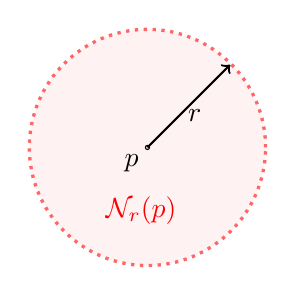
\begin{tikzpicture}
\filldraw[color=red!60, fill=red!5, very thick, dotted](0,0) circle (1.5);
\draw (0,0) circle [radius=0.75pt];
\draw [->, thick] (0,0) -- (1.05,1.05);
\draw (-0.2,-0.2) node {$p$};
\draw (0.6,0.4) node {$r$};
\draw (-0.08,-0.8) node [text=red] {$\mathcal{N}_r(p)$};
\end{tikzpicture}
\end{center}
% \end{wrapfigure}

Knowing the definition of a neighbourhood around a point, we can classify points based on these neighbourhoods as (for a point $p\in X$ and a subspace $E\subset X$):

\begin{enumerate}[label=D\arabic*.]
\item \textbf{Interior point:} $p\in X$ is an interior point of $E\subset X$ if $\exists\,r>0$ such that $\mathcal{N}_r(p)\subset E$.
\item \textbf{Limit point:} $p\in X$ is a limit point of set $E$ if \textit{every} neighbourhood of $p$ has a point $q\neq p$, i.e., $\left(\mathcal{N}_r(p)\setminus {p}\right) \cap E \neq \nullset$.
\item \textbf{Isolated point:} If $p\in E$ and $p$ is not a limit point, it is isolated.
\end{enumerate}

\subsection{Open \& Closed Sets}
We can also classify a set based on its constituent points as
\begin{enumerate}[label=S\arabic*.]
\item \textbf{Complement of a set:} If $E\subset X$, then its complement with respect to the metric space $X$ is $E^c=\{x\in X:x\notin E\}$
\item \textbf{Open set:} If all points of $E$ are interior points, it is an open set.
\item \textbf{Closed set:} If every limit point of $E$ is also a point in $E$, the set is closed
\item \textbf{Perfect set:} If $E$ is closed and every point of $E$ is a limit point, it is a perfect set.
\item \textbf{Bounded set:} If $\exists M\in \reals$ such that upon fixing $p\in E, d(p,x)<M\,\forall x\in E$, $E$ is bounded.
\item \textbf{Dense in $X$:}  If every $x\in X$ is a limit point of $E$, or a point of $E$ (or both), $E$ is dense in $X$.
\end{enumerate}

These definitions are abstractions of open intervals (open set), closed intervals (closed set), finite intervals (bounded set), `surfaces' of a set (closure), holes in an interval (isolated points), etc. These are very closely related to abstract intervals, to form continuums which are studied in topology. For instance, a limit point is closely related to sequences, as a limit point can be approximated by its neighbouring points.

Some properties of open and closed sets to be noted are:
\begin{enumerate}[label=(\roman*)]
\item $\nullset,X$ are open
\item If $E\subset X$ is open, then $E^c$ is closed.\\
This implies that $\nullset,X$ are both closed as well; finite sets are closed too because they have no limit points.
\item If $U,V\subset X$ are open sets, then $U \cup V$ is open.\\
Similarly, if $U,V\subset X$ are closed, then $U\cap V$ is closed (by (ii)).
\item More generally, if $\{U_\alpha\}_{\alpha\in A}$ are individually open $\forall \alpha\in A$, then $U=\bigcup\limits_{\alpha\in A} U_\alpha$ is open.\\
Using (ii), if $\{U_\alpha\}$'s are all closed for all $\alpha\in A$, $U=\bigcap\limits_{\alpha\in A} U_\alpha$ is closed.
\item $p$ is a limit point of $E$ iff $N_r(p)\cap E$ is infinite for any $r>0$.
\end{enumerate}

\begin{definition}
If $E\subset X$, then denote by $E'$ the set of all limit points of $E$, and by $\bar{E}=E\cup E'$. Then $\bar{E}$ is called the \textbf{closure} of $E$.
\end{definition}
The set $E$ is then closed iff $E=\bar{E}$ and clearly, $E\subset \bar{E}$, where the closure is a closed set. This means that the operation closure($\cdot$) on a set is idempotent, i.e., $\bar{E} = \overline{\bar{E}}$.
Also, for some $A_i\subset X$ for some $i=1,2,\cdots,n$ (finite), $\bar{\bigcup\limits^n_{i=1}A_i} = \bigcup\limits^n_{i=1}\bar{A_i}$, which can be proved by induction.

\section{Compact Sets}
A compact set abstracts the notion of mathematical infinities. Compact sets try to avoid infinities arising in two manners: a) infinite size of set (unboundedness), and b) infinities due to limit points not lying in the set (by making them `compact'). It is easier to understand what compactness means for a set by first defining a compact set, and then seeing relaxing which other properties makes a set non-compact.

\begin{definition}[Open Cover]
Consider a set $E\subset X$. If there exists a collection of open sets $G=\{G_\alpha\}$ such that $E\subset \bigcup\limits_{\alpha\in A}G_\alpha$, then $G$ is an open cover of $E$.
\end{definition}
\begin{definition}[Compact Set]
A set $E\subset X$ is compact if \textbf{every} open cover of $E$ has a finite subcover of $E$.
\end{definition}

So, if I have to prove a set is non-compact, I only need to find one counter example of an open cover of $E$ that does not contain a subcover of $E$.
On the other hand, to prove a set is compact is harder, because \textbf{every} open cover needs to have a finite subcover. For example, consider $E=\{1/n:n=1,2,\cdots\}$, is not compact. I can easily prove this by considering an open cover of the form $G_n=(1-1/n,1+1/n)$, which is a series of shrinking intervals centred around 1. But the limit point of $E$, which is $0$, never lies in a finite subcover.
Later on we will see that using Heine-Borel theorem requires this set to be closed in order to be compact, which it is not, since $0\notin E$.
On the other hand $E=\{1/n:n=1,2,\cdots\}\cup\{0\}$ is compact.

It is easier to understand what compactness means if we try to see how we can make a set non-compact. One obvious way to do so is by making the set so large that no finite subcover contains it. That is, \textit{make the set unbounded}. Consider a set $E=\{x\in \reals : x\geq0\}$. The infimum $0\in E$, but since the set is infinite in size, i.e., $\nexists M \in \reals$ such that $d(x,p)<M\,\forall x\in E$ for a fixed point $p$. This set is trivially noncompact. On the other hand, consider the set $E=(a,b)\subset\reals$. Despite the finite `size' of the interval (bounded trivially by $|b-a|$),the interval is not compact because it struggles with an infinity of the second kind.

\begin{center}
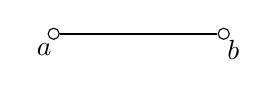
\begin{tikzpicture}
\draw (-0.08,0) circle [radius=2pt];
\draw (2.08,0) circle [radius=2pt];
\draw [thick] (0,0) -- (2,0);
\draw (-0.2,-0.2) node {$a$};bol
\draw (2.2,-0.2) node {$b$};
\end{tikzpicture}
\end{center}

This set has issues related to infinities of a different sort. No matter how close you approach to the limit point $a$ (or $b$), you never reach there, as it is not in your set. In fact, $(a,b)$ is topologically similar to $(-\infty,\infty)$! \\
An important thing to note, which is often confused, is that \textbf{every} open cover should have a finite subcover for a set to be compact. It is harder to prove compactness, and easier to prove noncompactness, as the latter requires one counter example of an open cover not having a finite subcover. Similarly, simply finding one open cover that has an open subcover leads to nothing. For instance, recall that the metric space $X$ is open (and also closed). So $X$ covers literally every subset of $X$! But that does not mean every subset of $X$ is compact, as compactness requires all open covers to have a finite subcover.\\

\begin{lemma}
\begin{enumerate}
\item Compact subsets of metric spaces are closed
\item Closed subsets of compact sets are compact
\end{enumerate}
\end{lemma}
\begin{corollary}
If $F$ is a closed set and $K\subset X$ a compact set, then $F\cap K$ is compact.
\end{corollary}

This also leads us naturally to the Heine-Borel Theorem. Recall from the discussion above that to make a set compact, we need to `fix' the two kinds of infinities we encountered. The first one is fixed by making our set small enough for there to be even a possibility of a finite (sub)cover, i.e., boundedness. The other fixes the existence of limit points, which introduce infinities around them, i.e., closed sets.

\begin{theorem}[Heine-Borel Theorem]
$K\subset \reals^k$ is compact $\iff K$ is closed and bounded. \textbf{note that this is only for Euclidean spaces}.
\begin{lemma}
Closed subsets of compact sets are compact.
\end{lemma}
\begin{lemma}
Closed $k-$cells in $reals^k$ are compact.
\end{lemma}
\end{theorem}

\begin{theorem}[Bolzano-Weierstrass Theorem]
Let $K\subset X$ be a compact set, and $E\subset K$ an infinite subset of $K$, them $E$ has a limit point in $K$.
\end{theorem}

\begin{theorem}[Kantor Intersection Theorem]
If $K_n\subset X$ is a sequence of nonempty compact sets such that $K_n\supset K_{n+1}$ for $n=1,2,\cdots$, then $\bigcap\limits_{i=1}^{\infty}K_i \neq \nullset$.
\end{theorem}

\subsection{Perfect Sets}
\begin{definition}
A nonempty set $P\subset X$ is a \textbf{perfect} set if $P$ is closed and all points $P$ are limit points of $P$, or if $P$ is closed and has no isolated points.
\end{definition}
\begin{theorem}[Perfect sets are uncountable]
If $P\subset \reals^k, P\neq \nullset$ is a perfect set, then $P$ is uncountable.
\end{theorem}

\subsection{Connected Sets} 
Two disjoint sets $A,B\subset X$  are \textbf{separated} if $\bar{A}\cap B\neq \nullset$ and ${A}\cap \bar{B}\neq \nullset$. We say that $E$ is \textbf{disconnected} if $\exists\, A,B$ such that $A,B\neq \nullset$, $A,B$ are separated, and $E=A\cup B$. Finally, a set $E\subset X$ is connected if it is not disconnected.\\
The concept of connectedness says that the set $E$ should not be breakable into two sets `far apart'. The notion of `far apart' is conveyed by the set being breakable into two open sets.

\begin{theorem}[Connected sets in $\reals$]
A set $E\subset \reals$ is connected iff it has the \textbf{interval property}: if $x,y\in E$, then $[x,y]\in E$ for some $x<y$.
\end{theorem}

\begin{lemma}
If $V\subset \reals$ is bounded above and $V\neq \nullset$, then $\sup{V}\in \bar{V}$.
\end{lemma}